\documentclass{article}

\usepackage[utf8]{inputenc}
\usepackage[T1]{fontenc}
\usepackage{lipsum}
\usepackage{graphicx}
\usepackage{amsmath}
\usepackage[margin=1in]{geometry}
\usepackage{titlesec}
\usepackage{parskip}
\usepackage{tcolorbox}

\titleformat{\section}
{\LARGE\bfseries}{\thesection}{1em}{}

\titleformat{\subsection}
{\Large\bfseries}{\thesection}{1em}{}

\begin{document}

\pagestyle{empty}

\section*{Monadi}
\large

Una delle caratteristiche principali di Haskell è l'essere un linguaggio \textbf{lazy}.

Questa caratteristica porta ad alcune conseguenze positive, come:
\begin{itemize}
    \item Purezza: in un linguaggio completamente puro è presente la \textbf{trasparenza referenziale}.
    
    La trasparenza referenziale si può definire come: 
    
    \begin{center}
        Se \texttt{a = b} posso usare \texttt{a} al posto di \texttt{b} e viceversa.
    \end{center}

    Un possibile esempio di questo concetto può essere:
\begin{tcolorbox}
\begin{verbatim}
f x = a + a
    where
        a = g x
        b = h 3
\end{verbatim}
\end{tcolorbox}

    il quale viene tradotto dal compilatore Haskell in:
\begin{tcolorbox}
\begin{verbatim}
f x = g x + g x
\end{verbatim}
\end{tcolorbox}

    E' quindi possibile osservare come \texttt{a} venga sostituita con la sua definizione sottostante (ottimizzazione, \textbf{inlining}), andando a rimuovere completamente la definizione di \texttt{b} (non utilizzata).

    Questo è possibile solo se il linguaggio è puro, dove non è possibile alterare lo stato esterno.

    Se il linguaggio non fosse stato puro, \texttt{g} ed \texttt{h} avrebbero potuto causare effetti collaterali con la loro esecuzione. In questo caso, la traduzione effettuata dal compilatore non sarebbe stata corretta.
    \item Modularità dei programmi: è possibile dividere il programma in moduli differenti, richiamati solo se strettamente necessario.
    \item Normalizzazione (ad esempio, nel caso della funzione \texttt{const 1 undefined}, dove \texttt{undefined} non verrà mai valutato perché non utilizzato).
    \item Parallelismo: nei linguaggi pigri, e di conseguenza puri, è semplice parallelizzare l'esecuzione.
\end{itemize}
ma anche conseguenze negative, come:
\begin{itemize}
    \item Purezza: in un linguaggio completamente puro non è possibile stampare a schermo, stabilire connessioni di rete, ecc. Questo rende il linguaggio abbastanza inutile.
    \item Imprevedibilità: ad esempio, nel caso della funzione \texttt{const (print 1) (print 2)}, non si riesce a capire guardando solamente il codice quale sarà l'esito dell'esecuzione.
\end{itemize}

Un possibile esempio di purezza come conseguenza negativa in Haskell è la gestione di Input/Output (dialoghi). Prima delle monadi, questo procedimento richiedeva una logica contorta.

\pagebreak

Prima di introdurre il concetto di \textbf{monade}, bisogna fare una distinzione tra il fare qualcosa rispetto al pensare di fare qualcosa.

Nella programmazione tradizionale viene scritto in maniera esplicita quello che il programma deve fare, passo dopo passo.

Nella programmazione con monadi, il progrmama \textbf{crea delle azioni che se eseguite hanno un effetto collaterale} (come una stampa a schermo).

Una possibile rappresentazione grafica di questo concetto può essere:\\
\begin{center}
    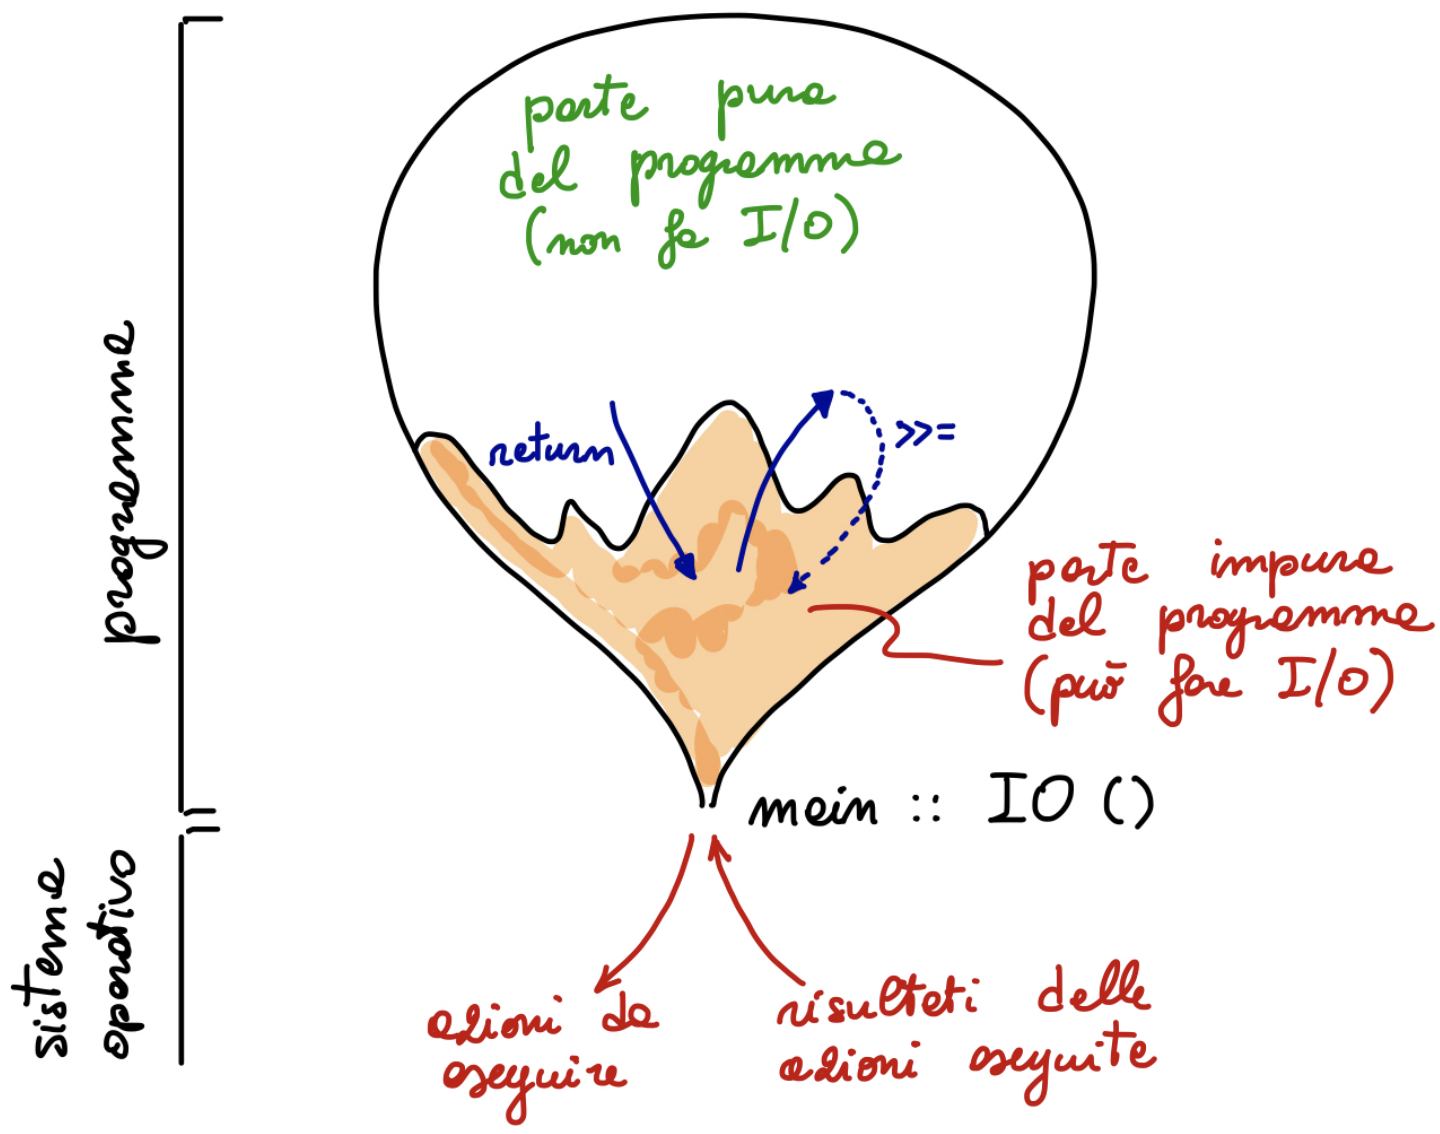
\includegraphics[width=0.8\textwidth]{img/monadi.png}
\end{center}

E' quindi presente una suddivisione tra la parte \textit{pura} e \textit{impura} del programma. Il nostro programma rimane puro, delegando al sistema operativo l'esecuzione di funzionalità impure.

Inizialmente l'idea delle monadi era stata pensata per gestire il problema dell'input/output. Successivamente ci si è resi conto che poteva essere utilizzata anche per altri scopi (alcuni possono essere eccezioni, parallelismo, transazioni).

Una monade può essere anche definita come: concetto nell’area della semantica dei linguaggi per descrivere matematicamente \textbf{computazioni} che possono avere \textbf{effetti collaterali}.

E' possibile trovare monadi anche in linguaggi moderni, come Scala e Javascript, fornendo un modo strutturato di organizzare computazioni con effetti collaterali.\vspace{14pt}\\
Di seguito vengono mostrati diversi esempi pratici di applicazione di monadi.

\pagebreak

\subsection*{Valutatore di espressioni}
Si vuole realizzare un valutatore per semplici espressioni aritmetiche.
\begin{tcolorbox}
\begin{verbatim}
data Expr = Const Int | Div Expr Expr

eval :: Expr -> Int
eval (Const n) = n
eval (Div t s) = eval t ‘div‘ eval s
\end{verbatim}
\end{tcolorbox}
\texttt{Expr} indica una struttura dati custom, la quale può avere un valore \texttt{Int} oppure rappresentare una espressione aritmetica.

Vengono successivamente definiti due casi possibili: restituzione del valore inviato e calcolo dell'espressione.

Si vuole ora raffinare il valutatore in modo che supporti:
\begin{itemize}
    \item Gestione delle \textbf{divisioni per zero}
    \item \textbf{Conteggio} delle operazioni “difficili”
    \item \textbf{Tracciamento} dei passi di valutazione
\end{itemize}
Se usassimo un linguaggio impuro sarebbe tutto facile.\vspace{14pt}\\
Partiamo dalla divisione per zero.\\
Per implementare la gestione della divisione per zero viene modificato il codice nel seguente modo:
\begin{tcolorbox}
\begin{verbatim}
eval :: Expr -> Maybe Int
eval (Const n) = Just n
eval (Div t s) =
    case eval t of
        Nothing -> Nothing
        Just m -> case eval s of
            Nothing -> Nothing
            Just 0 -> Nothing
            Just n -> Just (m ‘div‘ n)
\end{verbatim}
\end{tcolorbox}
Ciò che era facile fare in un linguaggio impuro ha stravolto la struttura del programma in un linguaggio puro. La logica del programma si perde nella gestione dell’eccezione.

Si passa ora al conteggio delle operazioni "difficili".\\
ciao

\end{document}